\section{Introduction}
\begin{figure*}[h]
\centering
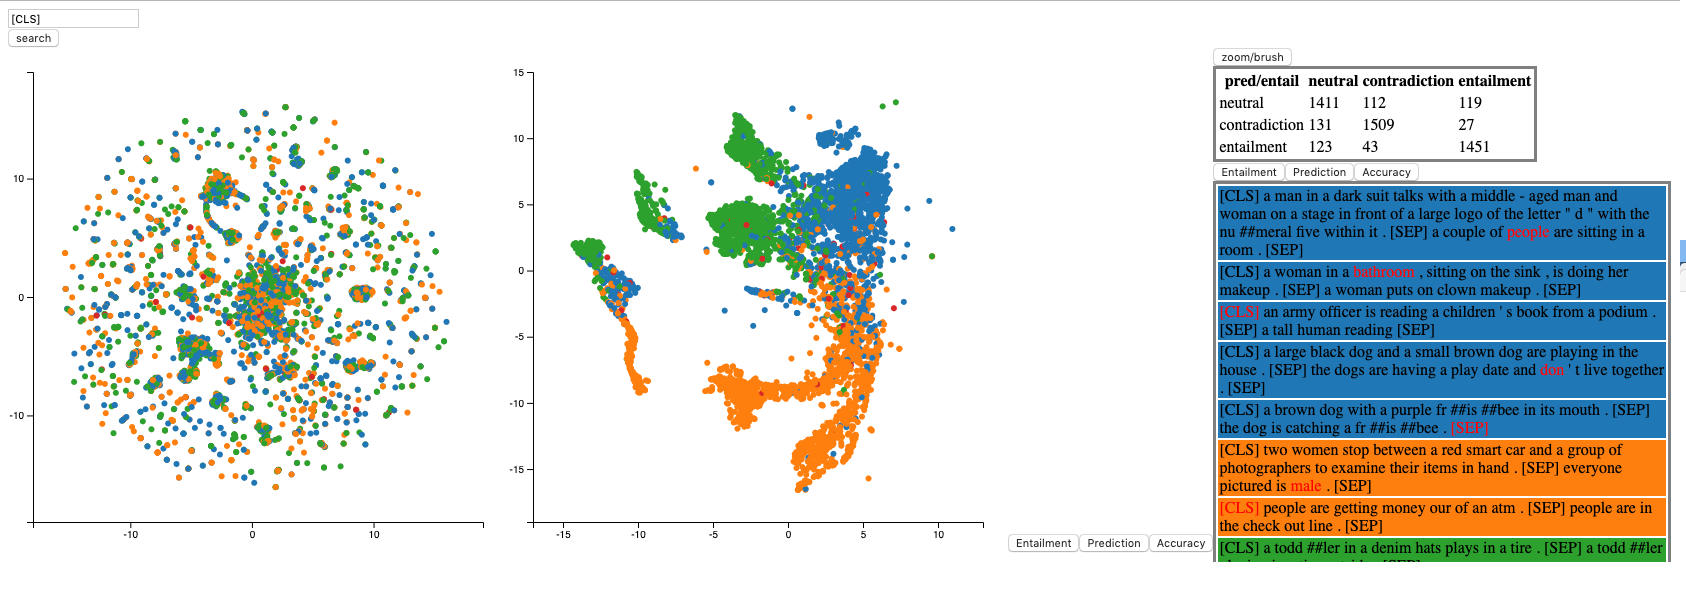
\includegraphics[width=.80\textwidth]{figs/fig1.png}
\vspace{-2mm}
\caption{
The overview of our UI, we sampled the points and show them in the scatterplots, the plot in the left is the word vectors before fine-tuning and the right one is after fine-tuning. The color indicates the label of the sentence pairs this word belongs to. Green means entailment, orange means contradiction and blue means neutral. We put a search bar in the UI, people can type any word they interested in and filter the scatterplots to only show the vectors for searched word. The statistic table shows statistics for selected points, if no selection, it will show the statistic for all words. We also sampled 10 sentences for selected word.
}
\label{fig:mainui}
%\vspace{-4mm}
\end{figure*}
Deep contextualized word representations like BERT or ELMo have achieved great success in many NLP fields. But not like the traditional embeddings like word2vec or glove, BERT vectors are based on its surroundings words, which means the embedding of the same word may differ from sentence to sentence. The good news of this kind of embeddings is they include the contextual information in the vectors and the experiments showed that it really improve the results for many tasks. But the bad news is it needs more resources and time to train the model and the embeddings are not re-usable since the embeddings are different in different sentences. In this project, I built an interactive UI for visualizing the BERT embeddings.